\documentclass{beamer}

\newcommand{\lesson}{Exceptions}

\newcommand{\course}{Introduction to Object-Oriented Programming}
\subject{\course}
\title[\lesson]{\course}
\subtitle{\lesson}

\author[CS 1331]
{Christopher Simpkins \\\texttt{chris.simpkins@gatech.edu}}
\institute[Georgia Tech]

\date[]{}

\newcommand{\link}[2]{\href{#1}{\textcolor{blue}{\underline{#2}}}}
\newcommand{\code}{http://www.cs1331.org/code}

\usepackage{colortbl}

% If you have a file called "university-logo-filename.xxx", where xxx
% is a graphic format that can be processed by latex or pdflatex,
% resp., then you can add a logo as follows:

% \pgfdeclareimage[width=0.6in]{coc-logo}{cc_2012_logo}
% \logo{\pgfuseimage{coc-logo}}

\mode<presentation>
{
  \usetheme{Berlin}
  \useoutertheme{infolines}

  % or ...

 \setbeamercovered{transparent}
  % or whatever (possibly just delete it)
}

\usepackage{tikz}
% Optional PGF libraries
\usepackage{pgflibraryarrows}
\usepackage{pgflibrarysnakes}
\usepackage{pgfplots}
\usepackage{fancybox}
\usepackage{listings}
\usepackage{hyperref}
\hypersetup{colorlinks=true,urlcolor=blue}
\usepackage[english]{babel}
% or whatever

\usepackage[latin1]{inputenc}
% or whatever

\usepackage{times}
\usepackage[T1]{fontenc}
% Or whatever. Note that the encoding and the font should match. If T1
% does not look nice, try deleting the line with the fontenc.


\usepackage{listings}

% "define" Scala
\lstdefinelanguage{scala}{
  morekeywords={abstract,case,catch,class,def,%
    do,else,extends,false,final,finally,%
    for,if,implicit,import,match,mixin,%
    new,null,object,override,package,%
    private,protected,requires,return,sealed,%
    super,this,throw,trait,true,try,%
    type,val,var,while,with,yield},
  otherkeywords={=>,<-,<\%,<:,>:,\#,@},
  sensitive=true,
  morecomment=[l]{//},
  morecomment=[n]{/*}{*/},
  morestring=[b]",
  morestring=[b]',
  morestring=[b]""",
}

\usepackage{color}
\definecolor{dkgreen}{rgb}{0,0.6,0}
\definecolor{gray}{rgb}{0.5,0.5,0.5}
\definecolor{mauve}{rgb}{0.58,0,0.82}

% Default settings for code listings
\lstset{frame=tb,
  language=scala,
  aboveskip=2mm,
  belowskip=2mm,
  showstringspaces=false,
  columns=flexible,
  basicstyle={\scriptsize\ttfamily},
  numbers=none,
  numberstyle=\tiny\color{gray},
  keywordstyle=\color{blue},
  commentstyle=\color{dkgreen},
  stringstyle=\color{mauve},
  frame=single,
  breaklines=true,
  breakatwhitespace=true,
  keepspaces=true
  %tabsize=3
}


% If you wish to uncover everything in a step-wise fashion, uncomment
% the following command:

% \beamerdefaultoverlayspecification{<+->}


\begin{document}

\begin{frame}
  \titlepage
\end{frame}

%------------------------------------------------------------------------
\begin{frame}[fragile]{Erorr Handling Code}

Consider this code from \link{\code/employee/Company.java}{Company.java}:
\begin{lstlisting}[language=Java]
  employees = initFromFile2(new File(empDataFile));
  if (null == employees) {
      System.out.println("There was an error initializing employees.");
      System.out.println("Perhaps " + empDataFile + " doesn't exist?");
      System.exit(1);
  }
\end{lstlisting}

\begin{itemize}
\item The main logic and error-handling logic are intertwined (not complex in this case, but could be much worse in other cases)
\item We have to remember to check for the sentinel value that indicates an error
\item We have to remember what the sentinel value is ({\tt null} in this case)
\item If we wanted to distinguish between different kinds of errors, we'd have to have multiple sentinel values
\item The compiler doesn't force us to handle errors
\end{itemize}


\end{frame}
%------------------------------------------------------------------------

%------------------------------------------------------------------------
\begin{frame}[fragile]{Exceptions}


An exception is
\begin{itemize}
\item an event that occurs during the execution of a program that disrupts the normal flow of instructions (\link{http://docs.oracle.com/javase/tutorial/essential/exceptions/index.html}{Java Tutorial - Exceptions});
\item a violation of the semantic constraints of a program;
\item an object that you create when an exception occurs.
\end{itemize}
\vspace{.1in}
An exception is said to be
\begin{itemize}
\item {\it thrown} from the point where it occurred and
\item {\it caught} at the point to which control is transferred (\href{http://docs.oracle.com/javase/specs/jls/se7/html/jls-11.html}{JLS \S 11}).
\end{itemize}
The basic syntax is:
\begin{lstlisting}[language=Java]
try {
    // Code that may throw an exception
} catch (Exception e) {
    // Code that is executed if an exception is
    // thrown in the try-block above
}
\end{lstlisting}
We'll

\end{frame}
%------------------------------------------------------------------------

%------------------------------------------------------------------------
\begin{frame}[fragile]{Using Exceptions}


Here's our previous example rewritten to use exceptions:
\begin{lstlisting}[language=Java]
try {
    employees = initFromFile(new File(employeeDataFile));
} catch (FileNotFoundException e) {
    System.out.println("Need an employee data file.");
    System.out.println(e.getMessage());
} ...
\end{lstlisting}
{\tt initFromFile()} declares that it {\tt throws FileNotFoundException} and some other exceptions:
\begin{lstlisting}[language=Java]
private List<Employee> initFromFile(File empData)
        throws FileNotFoundException, IOException, ParseException {
\end{lstlisting}

The fact that {\tt initFromFile} declares that it throws checked exceptions (more later) means {\tt javac} will require us to handle the exceptions.

\end{frame}
%------------------------------------------------------------------------

%------------------------------------------------------------------------
\begin{frame}[fragile]{{\tt try} Statements}


\begin{lstlisting}[language=Java]
try {
    initFromFile(new File(employeeDataFile));
} catch (FileNotFoundException e) {
    System.out.println("Need an employee data file.");
    System.out.println(e.getMessage());
} ...
\end{lstlisting}

\begin{itemize}
\item If {\tt initFromFile()} does throw a {\tt FileNotFoundException}, control is transferred to the catch block.
\item The {\tt FileNotFoundException} object that is thrown from {\tt initFromFile()} is bound to the variable {\tt e} in the catch block.
\item The absence of the specified file is a violation of a semantic constraint of the {\tt initFromFile} method (which it propagates from {\tt FileReader} - more later).
\end{itemize}
Now you know the basics.  Let's explore the details ...

\end{frame}
%------------------------------------------------------------------------


%------------------------------------------------------------------------
\begin{frame}[fragile]{Run-Time Exception Handling}


Throwing an exception causes a nonlocal transfer of control from the point where the exception is thrown to the nearest dynamically enclosing catch clause.
\begin{quote}
A statement or expression is dynamically enclosed by a catch clause if it appears within the try block of the try statement of which the catch clause is a part, or if the caller of the statement or expression is dynamically enclosed by the catch clause. -- \href{http://docs.oracle.com/javase/specs/jls/se7/html/jls-11.html#jls-11.3}{JLS \S 11.3}
\end{quote}
More simply, a statement is dynamically enclosed by a catch clause if it is
\begin{itemize}
\item contained within the corresponding try block of the catch clasuse, or
\item  within a method (or constructor) that is called within the corresponding try block of the catch clause.
\end{itemize}

\end{frame}
%------------------------------------------------------------------------

%------------------------------------------------------------------------
\begin{frame}[fragile]{Identifying a Dynamically Enclosing Catch Clause}


\begin{lstlisting}[language=Java,escapechar=`]
public Company(String employeeDataFile) {
    try {
        employees = initFromFile(new File(employeeDataFile));
    } `\colorbox{yellow}{catch (FileNotFoundException e) \{}`
        System.out.println("Missing employee file:" + e.getMessage());
    }
}
private void initFromFile(File empData) throws FileNotFoundException {
    BufferedReader reader =
        new BufferedReader(`\colorbox{yellow}{new FileReader(empData)}`);
}
\end{lstlisting}

The highlighted statement in {\tt initFromFile} is dynamically enclosed by the highlighted catch clause in the {\tt Company} constructor because it is within a method that is called within the coresposnding try block of the catch clause (and the statement within the {\tt FileReader} constructor that acutally throws the exception is also dynamically enclosed by the highlighted catch clause).



\end{frame}
%------------------------------------------------------------------------

%------------------------------------------------------------------------
\begin{frame}[fragile]{Catch Block Parameters}
\vspace{-.1in}
\begin{lstlisting}[language=Java,escapechar=`]
public Company(String employeeDataFile) {
    try {
        employees = initFromFile(new File(employeeDataFile));
    } `\colorbox{yellow}{catch (FileNotFoundException e) \{}`
        System.out.println("Missing employee file:" + e.getMessage());
    }
}
private void initFromFile(File empData) throws FileNotFoundException {
    BufferedReader reader =
        new BufferedReader(`\colorbox{yellow}{new FileReader(empData)}`);
}
\end{lstlisting}
\vspace{-.1in}
\begin{itemize}
\item If {\tt new FileReader(empData)} throws a {\tt FileNotFoundException}, it will be caught in the catch block and bound to the catch block's parameter {\tt e}.
\item The object {\tt e} has type {\tt FileNotFoundException} and can be used just like any other object.
\item {\tt FileNotFoundException} is a standard library exception, so you can look up its API documentation just like any other standard library class.
\end{itemize}

\end{frame}
%------------------------------------------------------------------------

%------------------------------------------------------------------------
\begin{frame}[fragile]{Java's Exception Hierarchy}

\begin{columns}[t]
\begin{column}{2in}
\begin{center}
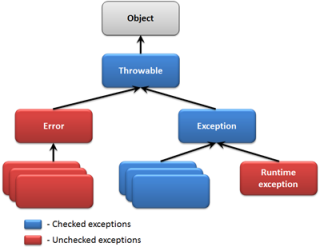
\includegraphics[height=2.5in]{hierarchy_of_java_exceptions.png}
\end{center}
\end{column}
\begin{column}{3in}
\begin{itemize}
\item Most (checked) exceptions will subclass {\tt Exception}
\item Most uncheked exceptions will subclass {\tt RuntimeException}
\item {\tt Error} is for compiler hackers.  Don't use it directly.
\end{itemize}
\end{column}
\end{columns}

\end{frame}
%------------------------------------------------------------------------



%------------------------------------------------------------------------
\begin{frame}[fragile]{Checked and Unchecked Exceptions}


Checked exceptions are subclasses of {\tt Throwable} that are not subclasses of {\tt RuntimeException} or {\tt Error}.  The compiler requires that checked exceptions declared in the throws clauses of methods are handled by:
\begin{itemize}
\item a dynamically enclosing catch clause, or
\item a {\tt throws} declaration on the enclosing method or constructor.
\end{itemize}
This rule is sometimes called ``catch or specify'' or ``catch or declare.''\\
\vspace{.1in}
Unchecked exceptions (subclasses of {\tt RuntimeException} or {\tt Error}) are not subject to the catch or declare rule.

\end{frame}
%------------------------------------------------------------------------

%------------------------------------------------------------------------
\begin{frame}[fragile]{Catch or Declare}


For example, here are the two ways to deal with the {\tt FileNotFoundException} thrown by {\tt initFromFile}.\\
\vspace{.1in}
Catch:
\vspace{-.05in}
\begin{lstlisting}[language=Java,escapechar=`]
public Company(String employeeDataFile) {
  // ...
  try {
    employees = initFromFile(new File(employeeDataFile));
  } `\colorbox{yellow}{catch (FileNotFoundException e) \{}`
    System.out.println(e.getMessage());
  }
}
\end{lstlisting}
Declare:
\vspace{-.05in}
\begin{lstlisting}[language=Java,escapechar=`]
public Company(String employeeDataFile) `\colorbox{yellow}{throws FileNotFoundException \{}`
  // ...
  initFromFile(new File(employeeDataFile));
}
\end{lstlisting}

\end{frame}
%------------------------------------------------------------------------

%------------------------------------------------------------------------
\begin{frame}[fragile]{Throwing Exceptions is a Control Flow Mechanism}


What does this code print?
\begin{lstlisting}[language=Java]
public class Wee {

    static void bar() throws Throwable {
        throw new Throwable("Wee!");
    }

    static void foo() throws Throwable {
        bar();
        System.out.println("Foo!");
    }

    public static void main(String[] args) {
        try {
            foo();
        } catch (Throwable t) {
            System.out.println(t.getMessage());
        }
        System.out.println("I'm still running.");
    }
}
\end{lstlisting}

\end{frame}
%------------------------------------------------------------------------


%------------------------------------------------------------------------
\begin{frame}[fragile]{Taking Advantage of Unchecked Exceptions}


We've been using the Scanner class without having to handle exceptions because its methods throw unchecked exceptions.  But we can make use of these exceptions to make our code more robust.
\begin{lstlisting}[language=Java]
Scanner kbd = new Scanner(System.in);
int number = 0;
boolean isValidInput = false;
while (!isValidInput) {
    try {
        System.out.print("Enter an integer: ");
        number = kbd.nextInt();
        // If nextInt() throws an exception, we won't get here
        isValidInput = true;
    } catch (InputMismatchException e) {
        // This nextLine() consumes the token that
        // nextInt() couldn't translate to an int.
        String input = kbd.nextLine();
        System.out.println(input + " is not an integer.");
        System.out.println("Try again.");
    }
}
\end{lstlisting}


\end{frame}
%------------------------------------------------------------------------

%------------------------------------------------------------------------
\begin{frame}[fragile]{Multiple Catch Clauses}


Two important points in writing multiple catch clauses for a try statement:
\begin{itemize}
\item The exception type in a catch clause matches subclasses.
\item The first catch clause that matches an exception is the (only) one that executes.
\end{itemize}
This means that you should order your catch clauses from most specific (most derived, lowest in exception class hierarchy) to least specific (highest in exception class hierarchy).


\end{frame}
%------------------------------------------------------------------------

% %------------------------------------------------------------------------
% \begin{frame}[fragile]{Common Mistakes in Multiple Catch Clauses}
%
%
% What's wrong with this code?
% \begin{lstlisting}[language=Java]
% try {
%   initFromFile(new File(employeeDataFile));
% } catch (Exception e) {
%   System.out.println("Something bad happened: " + e.getMessage());
% } catch (IOException e) {
%   System.out.println(e.getMessage());
%   e.printStackTrace(System.out);
%   System.exit(0);
% } catch (FileNotFoundException e) {
%   System.out.println("Can't run without an employee data file.");
%   System.out.println(e.getMessage());
%   System.exit(0);
% } catch (ParseException e) {
%   String msg = "Malformed data caused exception: " + e.getMessage();
%   System.out.println(msg);
%   System.out.println("Full stack trace:");
%   e.printStackTrace(System.out);
%   System.exit(0);
% }
% \end{lstlisting}
%
%
% \end{frame}
% %------------------------------------------------------------------------
%

% %------------------------------------------------------------------------
% \begin{frame}[fragile]{Principles of Exception Handling}
%
%
% \begin{itemize}
% \item Don't try to handle coding errors.
% \item Prefer exceptions from the standard library to creating your own.
% \item Name exceptions after the problem (not the thrower).
% \item Wrap exceptions when crossing an abstraction boundary.
% \item Store useful information in exception objects.
% \item Handle exceptions close to their origins, but ...
% \begin{itemize}
%   \item Assign exception-handling responsibility to objects that can handle the exceptions.
%   \item Don't ``eat'' exceptions (at the very least, log the exception).
%   \item If you can't handle an exception sensibly, propagate it (``when in doubt, throw it out'').
% \end{itemize}
% \end{itemize}
%
% See \url{http://wirfs-brock.com/PDFs/towards_xcptn_hndling.pdf} for more details.  We'll just touch on a few of these here.
%
% \end{frame}
% %------------------------------------------------------------------------
%
% %------------------------------------------------------------------------
% \begin{frame}[fragile]{Applying Exception Handling Principles}
%
%
% What's wrong with this constructor?
% \begin{lstlisting}[language=Java]
% public class Company {
%     private ArrayList<Employee> employees;
%
%     public Company(String employeeDataFile) {
%         try {
%             employees = initFromFile(new File(employeeDataFile));
%         } catch (FileNotFoundException e) {
%             System.out.println("Employee data file not found.");
%         } catch (ParseException e) {
%             System.out.println("Malformed data file: "+e.getMessage();
%         } catch (Exception e) {
%             System.out.println("Exception occurred: "+e.getMessage());
%         }
%     }
%     //...
% }
% \end{lstlisting}
%
% \end{frame}
% %------------------------------------------------------------------------

%------------------------------------------------------------------------
\begin{frame}[fragile]{Writing and Using Your Own Exceptions}


Define your own exception classes by subclassing {\tt Exception} (for checked exceptions) or {\tt RuntimeException} (for unchecked exceptions).

\begin{lstlisting}[language=Java]
public class MyException extends Exception {

    public MyException(String msg) {
        super(msg);
    }
}
\end{lstlisting}
And use them just like any other exception:
\begin{lstlisting}[language=Java]
if (checkProblem()) {
    throw new MyException("Oops!");
}
\end{lstlisting}

But remember: in most cases there is an Exception class in the standard library that you can use. Don't write your own exception classes unless you really need to.

\end{frame}
%------------------------------------------------------------------------

%------------------------------------------------------------------------
\begin{frame}[fragile]{Use The Most Specific Applicable Exception}


Recall our {\tt Company} constructor:
\begin{lstlisting}[language=Java]
try {
    employees = initFromFile(new File(employeeDataFile));
} catch (FileNotFoundException e) {
    //...
} catch (ParseException e) {
    //...
} catch (Exception e) {
    //...
}
\end{lstlisting}
With separate exceptions we can take more specific actions, e.g.:
\begin{itemize}
\item We can tell the user to check for the right file (FileNotFoundException).
\item We can tell the user that the data file is malformed (ParseException).
\end{itemize}


\end{frame}
%------------------------------------------------------------------------

%------------------------------------------------------------------------
\begin{frame}[fragile]{Final Thoughts}

\begin{itemize}
\item Use exceptions for their intended purpose: separating your core logic from the code that handles exceptional conditions.
\item Use exceptions judiciously (not too many).
\item Think about how you handle exceptions:
\begin{itemize}
\item have sound reasons for propagating exceptions you propagate
\item have sound reasons for catching exceptions where you catch them
\item recover if you can
\item store information in your exceptions to aid in debugging or error recovery by the user
\end{itemize}
\end{itemize}


\end{frame}
%------------------------------------------------------------------------

% %------------------------------------------------------------------------
% \begin{frame}[fragile]{}


% \begin{lstlisting}[language=Java]

% \end{lstlisting}

% \begin{itemize}
% \item
% \end{itemize}


% \end{frame}
% %------------------------------------------------------------------------


\end{document}
